\documentclass{article}
\usepackage{amsmath}
\usepackage{graphicx}
\usepackage{float}
\usepackage{geometry}
\geometry{a4paper, margin=1in}

\begin{document}

\section*{Question 3}

\textit{The following data represent measurements (in cm) of shell lengths collected from a deposit in Spain.}

\section*{1.}

Let the number of samples be:
\[
n = 33
\]

Let the data in ascending order be:
\[
x_1 = 1.23,\; x_2 = 2.77,\; \ldots,\; x_i,\; \ldots,\; x_n = 8.86,\quad i \in \{1, 2, \ldots, n\}
\]

Then we have the mean:
\[
\bar{x} = \frac{1}{n} \sum_{i=1}^n x_i = \frac{15\,984}{3\,300} \approx 4.844
\]

Then we have the variance:
\[
\sigma_x^2 = \frac{1}{n} \sum_{i=1}^n x_i^2 - \bar{x}^2 \approx 3.342
\]

We have the index of the median:
\[
i_m = \frac{n + 1}{2} = 17
\]

Then we have the median:
\[
m = x_{i_m} = 4.4
\]

\subsection*{Answer}

\begin{itemize}
    \item $\bar{x} = \frac{15\,984}{3\,300} \approx 4.844$
    \item $\sigma_x^2 \approx 3.342$
    \item $m = 4.4$
\end{itemize}

\section*{2.}

Let the second quartile be:
\[
Q_2 = m = 4.4
\]

As well as the index of the second quartile:
\[
i_{Q_2} = i_m = 17
\]

Then we have the index of the first quartile ($Q_1$) and the index of the third quartile ($Q_3$):
\[
\begin{aligned}
i_{Q_1} &= \frac{n}{4} + \frac{1}{2} = 8.75 \\
i_{Q_3} &= \frac{3}{4} n + \frac{1}{2} = 25.25
\end{aligned}
\]

Then we have the first quartile and the third quartile:
\[
\begin{aligned}
Q_1 &= \frac{x_{\lceil i_{Q_1} - \frac{1}{2} \rceil} + x_{\lfloor i_{Q_1} + \frac{1}{2} \rfloor}}{2} = x_9 = 3.58 \\
Q_3 &= \frac{x_{\lceil i_{Q_3} - \frac{1}{2} \rceil} + x_{\lfloor i_{Q_3} + \frac{1}{2} \rfloor}}{2} = x_{25} = 5.24
\end{aligned}
\]

Then we have the interquartile range (IQR):
\[
\mathrm{IQR} = Q_3 - Q_1 = 1.66
\]

\subsection*{Answer}

\[
\mathrm{IQR} = 1.66
\]

\section*{3.}

Let the minimum ($\mathrm{min}$) and the maximum ($\mathrm{max}$) be:
\[
\begin{aligned}
\mathrm{min} &= x_1 = 1.23 \\
\mathrm{max} &= x_n = 8.86
\end{aligned}
\]

Then we have the boxplot:

\begin{figure}[H]
    \centering
    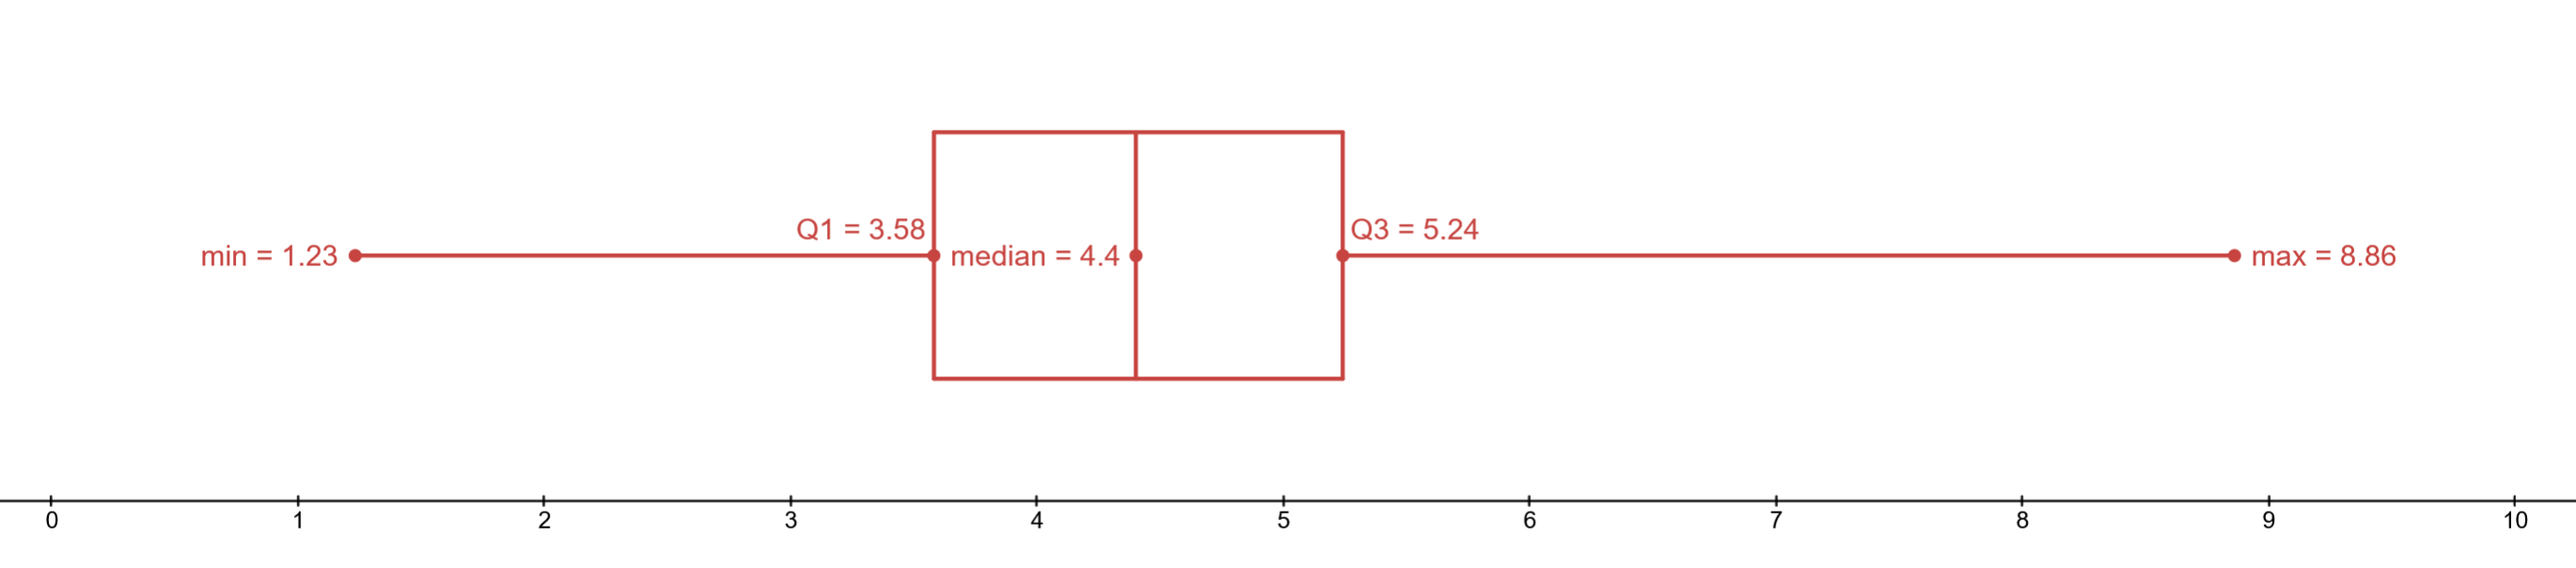
\includegraphics[width=1\textwidth]{Q3-P3-boxplot.png}
    \caption{Boxplot of shell lengths}
    \label{fig:boxplot}
\end{figure}

\subsection*{Answer}

\begin{figure}[H]
    \centering
    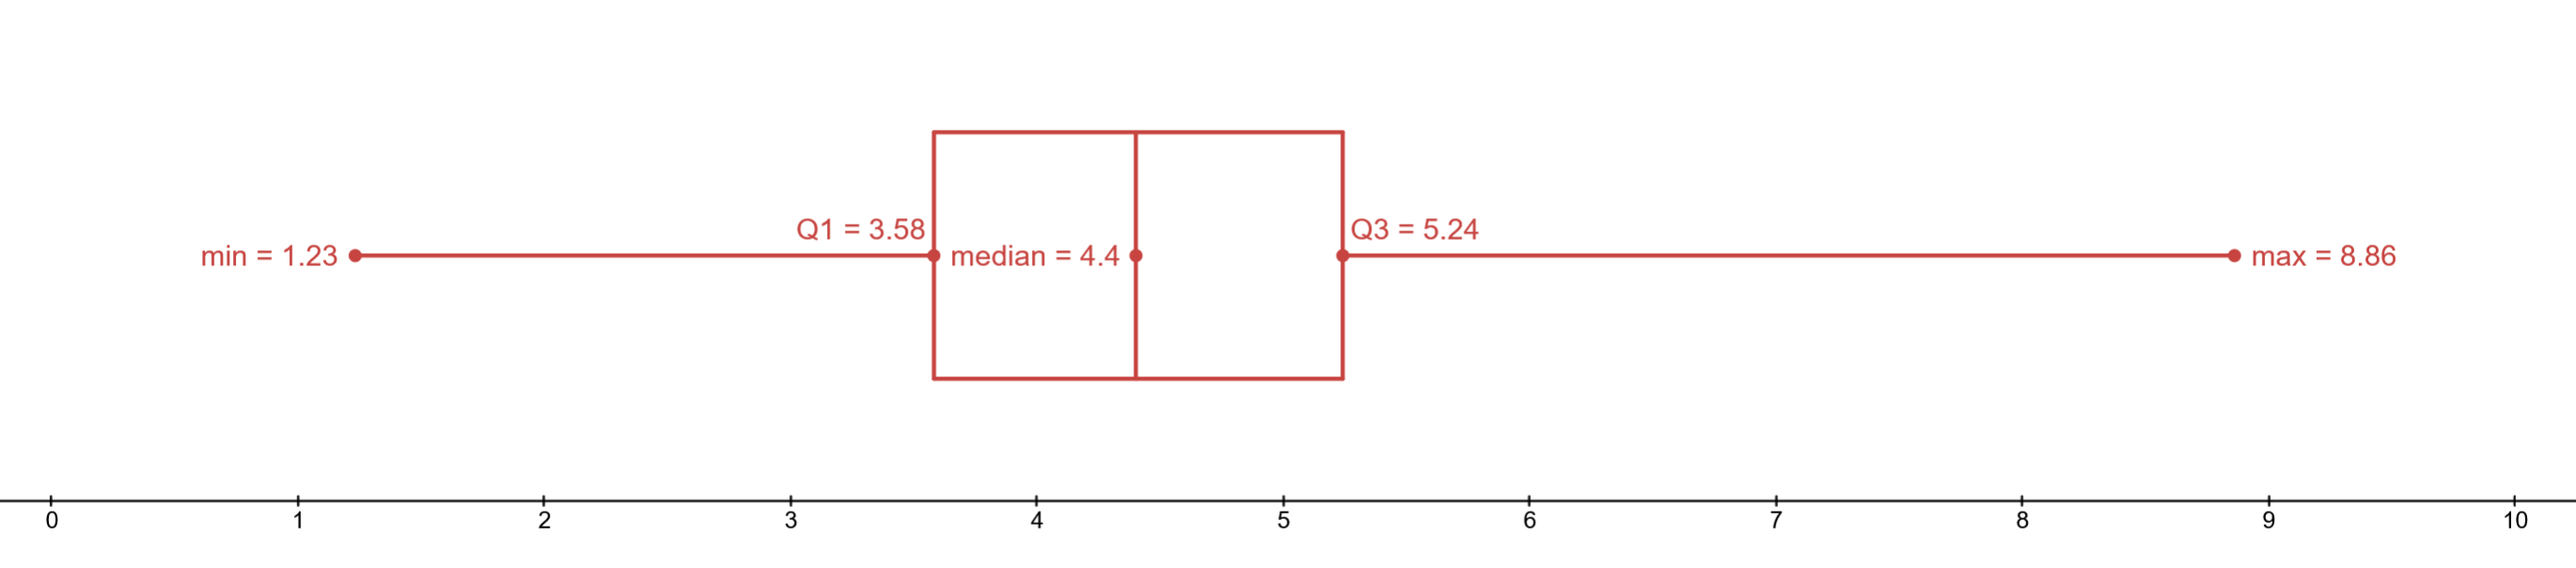
\includegraphics[width=1\textwidth]{Q3-P3-boxplot.png}
    \caption{Boxplot of shell lengths}
    \label{fig:boxplot}
\end{figure}

\end{document}
